\documentclass[11pt]{article}

\usepackage[spanish,activeacute]{babel}
\usepackage{titlesec}
\usepackage{graphicx}
\usepackage{float}
\usepackage[bottom]{footmisc}
\usepackage[hidelinks]{hyperref}
\usepackage{subcaption}
\usepackage[most]{tcolorbox}
\usepackage{xcolor}
\usepackage{listings}

\setlength{\parindent}{1.0em}
\setlength{\parskip}{1.0em}
\setlength{\emergencystretch}{5.0em}
\setlength{\belowcaptionskip}{-10pt}
\counterwithin{figure}{section}
\titlespacing*{\section}{0em}{3.5em}{1.5em}
\setcounter{tocdepth}{2}
\hypersetup{
	linktoc=all
}

\lstdefinestyle{HTML}{
	backgroundcolor=\color{white}, 
	basicstyle=\ttfamily\footnotesize,
	keywordstyle=\color{blue}\bfseries,
	commentstyle=\color{darkgray}\ttfamily,
	ndkeywordstyle=\color{green-html}\bfseries,
	stringstyle=\color{string-html},
	breakatwhitespace=false,
	breaklines=true,
	captionpos=b,
	keepspaces=true,
	numbers=left,
	numbersep=5pt,
	showspaces=false,
	showstringspaces=false,
	showtabs=false,
	tabsize=2
}

\title{\Huge Servidores}
\author{Eugenia Damonte, Ariel Fideleff y Mart\'in Go\~ni}
\date{}


\definecolor{light-orange}{RGB}{168,87,0}
\definecolor{light-blue}{RGB}{64, 76, 201}
\definecolor{dark-gray}{RGB}{100,100,100}
\definecolor{light-red}{RGB}{201, 60, 60}
\definecolor{fuchsia}{RGB}{168,0,168}
\definecolor{string-html}{rgb}{1, 0.5, 0}
\definecolor{green-html}{rgb}{0, 0.5, 0}


\newtcolorbox{code-box}{colback=white!75!gray,colframe=white!15!gray,fontupper=\linespread{1.15}\selectfont}


\newcommand{\imagecaption}[1]{\vspace{-7pt}\caption*{\char91\ref{fig:#1}\char93}}
\newcommand{\codetext}[2]{\large\texttt{\textcolor{#1}{#2}}}


\begin{document}
	\pagenumbering{gobble}
	\maketitle
	\newpage
	\tableofcontents
	\newpage
	\pagenumbering{arabic}
	
	
	\section{puTTY}
	\subsection{Que es puTTY}
		\texttt{puTTY} es una serie de herramientas de c'odigo abierto que permite la transferencia de archivos mediante la red, as'i como tambi'en el acceso a una consola serial, entre otras cosas. Cuando se habla de puTTY de manera general en realidad se est'a hablando de una serie de programas o componentes, desarrollados y mantenidos por el programador brit'anico Simon Tatham. Estos son:
		
		\begin{itemize}
			\item \texttt{puTTY} - Aplicaci'on para utilizar Telnet\footnote{Telnet o \texttt{Teletype Network} es un protocolo de red que permite acceder a la terminal de otra m'aquina de manera remota. Es adem'as el nombre del programa que usa el cliente.}, Rlogin\footnote{Rlogin o \texttt{Remote Login} es una aplicaci'on TCP/IP que inicia una sesi'on de terminal remota en el host especificado.} y un cliente SSH\footnote{Un cliente SSH es un programa que permite establecer conexiones seguras a servidores SSH.}, tambi'en permite la conexi'on a puertos seriales.
			\item \texttt{PSCP} - Cliente que permite realizar \textit{command-line secure file copy}, es decir copiar archivos de manera segura desde un terminal. Puede adem'as hacer transferencias SFTP.
			\item \texttt{PSFTP} - Cliente que permite utilizar SFTP\footnote{SFTP o \texttt{SSH File Transfer Protocol} es un protocolo seguro de transferencia de archivos, hoy en dia ha reemplazado casi completamente a FTP, su predecesor.} para transferir archivos.
			\item \texttt{puTTYtel} - Un cliente espec'ifico para Telnet.
			\item \texttt{Plink} - Una interfaz de consola que permite acceder a el \textit{back end} de puTTY. Normalmente usado para manejar t'uneles SSH\footnote{Un tunel SSH es un m'etodo para transportar informaci'on en la red de manera segura usando una conexi'on SSH encriptada.}.
			\item \texttt{Pageant} - Un agente de autenticaci'on para puTTY, PSCP y Plink.
			\item \texttt{puTTYgen} - Una aplicaci'on que permite generar llaves de encripci'on \texttt{RSA}, \texttt{DSA}, \texttt{ECDSA} y \texttt{EdDSA}.
		\end{itemize}
		
		En nuestro caso estamos interesados solamente en \texttt{puTTY} y \texttt{puTTYgen}, dado que son los necesarios para acceder de manera segura a una m'aquina remota usando SSH.
		
	
	\subsection{Conexi'on inicial}
		Nuestro objetivo con \texttt{puTTY} era usarlo para poder acceder de manera remota a una m'aquina\footnote{En nuestro caso utilizamos nuestra propia m'aquina virtual con \texttt{Debian 7}.} utilizando el protocolo SSH.
				
		Lo primero que hicimos fue crear un puerto por el cual pudi'esemos acceder a la \texttt{VM}, para hacer esto fuimos a la configuraci'on de la misma en \texttt{VirtualBox} y en el men'u \texttt{Network} abrimos las opciones avanzadas, seleccionando \texttt{Port Forwarding}. En el clickeamos el bot'on con el signo mas para crear una nueva regla de redirecci'on de puertos. Le pusimos \texttt{SSH} de nombre, dejando el protocolo en \texttt{TCP}. \texttt{Host IP} y \texttt{Guest IP} los dejamos vac'ios para que se asignen autom'aticamente al momento de uso, dado que las direcciones IP no son est'aticas. Finalmente completamos los campos correspondientes con los puertos. Para el del \texttt{Host}, es decir el de Windows, utilizamos el 5999 dado que es un puerto raro, haciendo poco probable que est'e ocupado. Para el puerto del \texttt{Guest}, es decir la VM, usamos el 22, el puerto est'andar usado por SSH.
		
		\begin{figure}[H]
    			\centering \captionsetup{justification=centering}
    			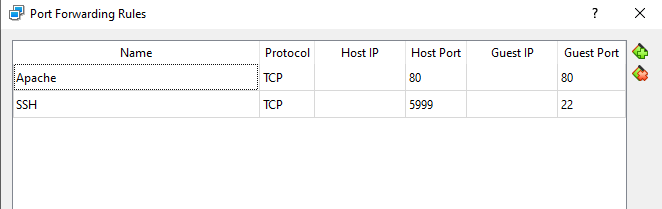
\includegraphics[scale=0.65]{Images/Install/port_forwarding.PNG}
    			\caption{El men'u de \texttt{port forwarding} de nuestra m'aquina virtual.}
    			\label{fig:port_forwarding}
		\end{figure}
		
		Una vez configurados los puertos nos dirigimos a la VM para verificar que los servicios SSH estuviesen funcionando de manera correcta. Para hacer esto usamos dos comandos, el primero \texttt{ps ax | grep ``ssh''} busca procesos con la palabra ``ssh'' en la lista de procesos activos. Al ejecutarlo encontr'o dos, indicando que los servicios estaban funcionando. Luego, para estar seguros utilizamos otro comando \texttt{/etc/init.d/ssh status}, al ejecutarlo nos inform'o, de nuevo, que los servicios SSH estaban funcionando correctamente. 
		
		\begin{figure}[H]
    			\centering
    			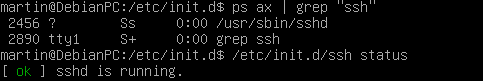
\includegraphics[scale=0.8]{Images/Config/SSH_check.PNG}
    			\caption{Los comandos usados para verificar el funcionamiento de los servicios SSH.}
    			\label{fig:SSH_check}
		\end{figure}
		
		Sabiendo que los servicios SSH estaban funcionando procedimos a realizar el primer intento de conectarnos de manera remota a la VM. Para hacer esto abrimos \texttt{puTTY}, y en el men'u \texttt{Session} pusimos \texttt{localhost} en \texttt{Host Name} y 5999 en \texttt{Port}. El resto de las opciones las dejamos con sus valores predeterminados. Lo que significan estos valores es dentro de la computadora misma (\texttt{localhost}), conectarse al puerto 5999, que es el que especificamos en la configuraci'on de la VM, usando el protoclo SSH.
		
		\begin{figure}[H]
    			\centering
    			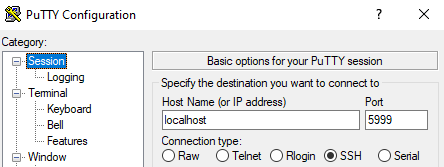
\includegraphics[scale=0.9]{Images/Connection/first_connection_attempt.PNG}
    			\caption{La configuraci'on para la primera conexi'on a la VM.}
    			\label{fig:first_connection_attempt}
		\end{figure}
		
		Habiendo ingresado toda la informaci'on clickeamos el bot'on \texttt{Open} para iniciar la conexi'on con la VM. Al hacerlo apareci'o una consola pidiendo que ingresemos nuestro nombre de usuario, y luego contraseña. Al ingresarlos, se nos concedi'o acceso, pudiendo usar la consola de \texttt{puTTY} como si fuese la consola de la VM. 
		
		\begin{figure}[H]
    			\centering
    			\captionsetup{justification=centering}
    			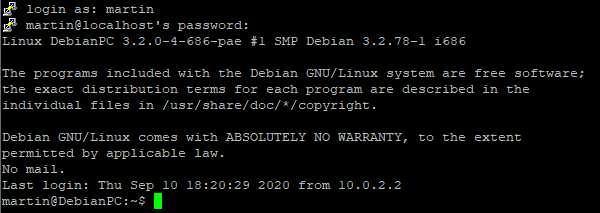
\includegraphics[width=0.9\linewidth]{Images/Connection/first_connection_console.PNG}
    			\caption{La primera conexi'on a la VM, hecha usando el protocolo SSH y \texttt{puTTY}.}
    			\label{fig:first_connection_console}
		\end{figure}
		
	\subsection{Conexi'on usando llaves}
		Si bien este m'etodo funciona, ser'ia muy peligroso usarlo para un servidor real. Esto es porque cualquiera podria conectarese a el mismo y obtener acceso al terminal de la m'aquina. Para solucionar este problema usamos una opci'on que tiene el protocolo SSH que permite validar conexiones mediante el uso de un par de llaves de encriptaci'on, una p'ublica y una privada. La p'ublica se encuentra en la VM, y la privada en la computadora desde la cual se realiza la conexi'on, siendo usada por \texttt{puTTY}.
		
		Lo primero que hay que hacer para usar la autenticaci'on por llaves es generarlas, por lo que para esto usamos el prgrama \texttt{puTTYgen}. Una vez abierto bajo la secci'on \texttt{Actions} clickeamos el bot'on \texttt{Generate} sin cambiar niguna de las opciones. Para que el par generado sea lo m'as aleatorio posible, puTTYgen nos dice que movamos el mouse de forma aleatoria por la ventana. Al terminar guardamos la llave privada como \texttt{id\_rsa.ppk} y la p'ublica como \texttt{public\_key} (con los botones \textit{Save private key} y \textit{Save public key} respectivamente).
		
		\begin{figure}[H]
    			\centering
    			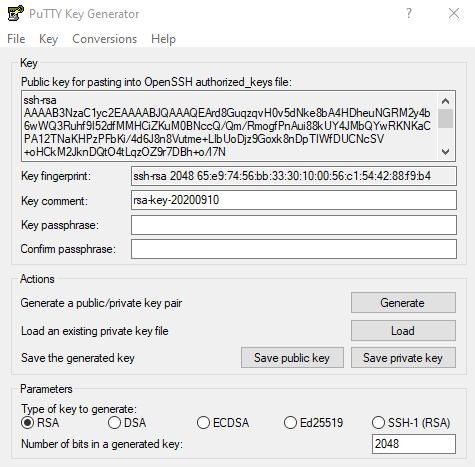
\includegraphics[scale=0.9]{Images/Connection/puTTYgen.PNG}
    			\caption{Configuraci'on de \texttt{puTTYgen} usada para generar las llaves.}
    			\label{fig:puTTYgen}
		\end{figure}
		
		Una vez generadas las llaves ten'iamos que llevar la p'ublica a la VM, as'i como tambi'en cambiar la configuraci'on de SSH para que solo permitiese conexiones con llaves. Para hacer esto volvimos a conectarnos a la VM usando \texttt{puTTY}. Una vez all'i lo primero que hicimos fue ir al directorio escondido \texttt{.ssh} en nuestro directorio propio (de no existir, podemos f'acilmente crearlo haciendo uso de \texttt{mkdir}). All'i creamos un archivo llamado \texttt{authorized\_keys}, en el copiamos la llave p'ublica generada por \texttt{puTTYgen}. 
		
		\begin{figure}[H]
    			\centering
    			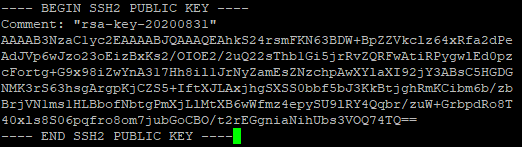
\includegraphics[scale=0.9]{Images/Connection/public_key.PNG}
    			\caption{Llave p'ublica copiada a la VM usando la terminal de \texttt{puTTY}.}
    			\label{fig:public_key}
		\end{figure}
		
		Con la llave p'ublica en la VM era hora de configurar SSH para que solo sea posible la autenticaci'on mediante llaves, no permitiendo usar contrase'nas (las de los usuarios del sistema, de la VM en nuestro caso). Para esto abrimos el archivo \texttt{/etc/ssh/sshd\_config} que es el archivo de configuraci'on de SSH. En 'el cambiamos cuatro cosas:
		
		\begin{itemize}
			\item Cambiamos \texttt{PubkeyAuthentication} de \texttt{no} a \texttt{yes}.
			\item Descomentamos \texttt{AuthorizedKeyFile \qquad \%h/.ssh/authorized\_keys}.
			\item Cambiamos \texttt{PasswordAuthentication} de \texttt{yes} a  \texttt{no}.
			\item Cambiamos \texttt{ChallengeResponseAuthentication} de \texttt{yes} a \texttt{no}.
		\end{itemize}
		
		Destacar que en caso de suceder que en cualquiera de las l'ineas cambiadas, est'a tambi'en comentada (es decir, que comienza con un \#), tambi'en descomentarla (quitando el \#). Para que estos cambios tomen efecto tuvimos que reiniciar los servicios SSH, usando el comando \texttt{sudo /etc/init.d/ssh restart}. Al ejecutarlo nos dijo que los servicios se hab'ian reiniciado correctamente.
		
		\begin{figure}[H]
    			\centering
    			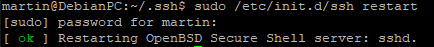
\includegraphics[scale=0.9]{Images/Connection/ssh_restart.PNG}
    			\caption{El comando usado para reiniciar los servicios SSH.}
    			\label{fig:ssh_restart}
		\end{figure}
		
		Para verificar si esto hab'ia funcionado primero era necesario configurar \texttt{puTTY} para utlizar la llave privada. Para hacerlo cerramos la terminal y volvimos a iniciar \texttt{puTTY}. En el men'u \texttt{Session} volvimos a introducir la misma informaci'on que antes. Luego fuimos al men'u \texttt{Data} bajo \texttt{Connection} donde en \texttt{Auto-login username} pusimos el nombre de usuario con el que queremos iniciar sesi'on en la VM. Finalmente fuimos a el submen'u \texttt{Auth}, bajo el men'u \texttt{SSH}, que tambi'en est'a en \texttt{Connection} y especificamos la ubicaci'on de la llave privada. Para hacer m'as r'apido el conectarse a la VM con \texttt{puTTY} guardamos todas las configuraciones en una sesi'on que llamamos \texttt{Debian 7 2}.
		
		\begin{figure}[H]
			\centering
			\begin{subfigure}[b]{0.45\linewidth}
				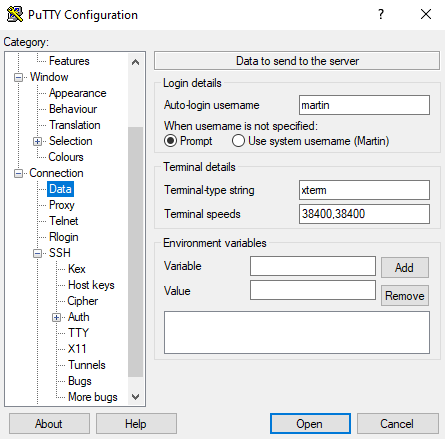
\includegraphics[scale=0.48]{Images/Connection/putty_data.PNG}
			\end{subfigure}
			\begin{subfigure}[b]{0.45\linewidth}
				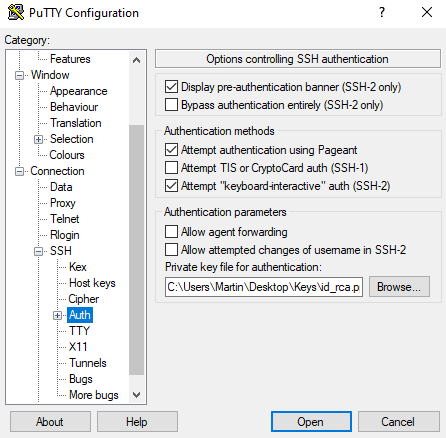
\includegraphics[scale=0.48]{Images/Connection/putty_SSH.PNG}
			\end{subfigure}
			\caption{Configuraci'on de los men'us \texttt{Data} y \texttt{Auth}.}
			\label{fig:putty_configs}
		\end{figure}
		
		Cuando terminamos de ingresar toda la informaci'on apretamos el bot'on \texttt{Open} para conectarnos con la VM. Mientras se establecia la conexi'on apareci'o una ventana de \texttt{puTTY} diciendo que hab'ia ocurrido un error. Este dec'ia \textit{No supported authentication methods available}, que se traduce como ``No hay metodos de autenticaci'on soportados disponibles''. Esto nos parecio extra'no ya que parec'ia que hab'iamos configurado todo correctamente y no hab'ia mucha informaci'on sobre cu'al era la causa del error.
		
		\begin{figure}[H]
    			\centering
    			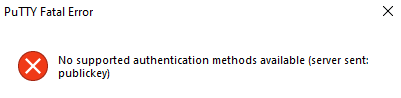
\includegraphics[scale=0.8]{Images/Connection/puTTY_error.PNG}
    			\caption{El error que nos di'o \texttt{puTTY} al intentar conectarnos.}
    			\label{fig:puTTY_error}
		\end{figure}
		
		Luego de investigar un poco descubrimos que la causa del error era c'omo hab'iamos ingresado la llave p'ublica. El formato correcto es \texttt{ssh-rsa (llave)}, estando todo en una misma l'inea.
		
		\begin{figure}[H]
    			\centering
    			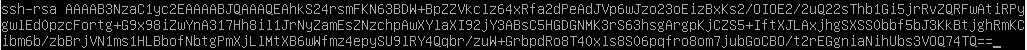
\includegraphics[scale=0.5]{Images/Connection/public_key_final.PNG}
    			\caption{}
    			\label{fig:public_key_final}
		\end{figure}
		
		Notar que, de hecho, cuando generamos las llaves, puTTYgen en un cuadro ya nos dejaba a disposici'on el texto que podr'iamos haber copiado y directamente pegado en el archivo \texttt{authorized\_keys}, en el formato correcto tal que sea reconocido por SSH, sin la necesidad de darle el formato por nuestra cuenta desde el archivo con la llave pública.
		
		Luego de solucionar ese problema intentamos conectarnos nuevamente a la VM, cosa que esta vez fue exitosa. Dado que hab'iamos podido conectarnos correctamente a nuestra VM desde \texttt{puTTY} utilizando las llaves, decidimos que ya estabamos listos para seguir con el pr'oximo paso, hacer un servidor con Apache.
		
		\begin{figure}[H]
    			\centering
    			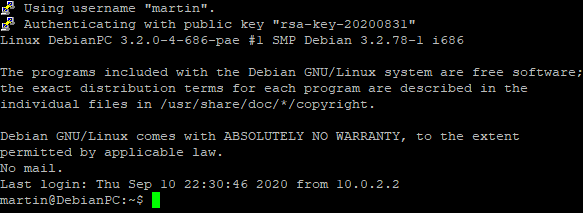
\includegraphics[scale=0.75]{Images/Connection/final_connection.PNG}
    			\caption{Nos conectamos de manera exitosa a la VM.}
    			\label{fig:final_connection}
		\end{figure}
		
		%%%
		
	\section{Servidor web}

		En esta instancia, decidimos instalar y configurar un servidor web: \texttt{Apache HTTP Server}. Un servidor web es un software que permite que un usuario pueda ver el contenido de una p'agina web. A grandes rasgos, lo que sucede al buscar una direcci'on en el navegador es que este busca en qu'e servidor o host se encuentra guardada la p'agina y le ``pide'' el contenido. El servidor web (que est'a instalado en el host) es el encargado de entreg'arselo.
		
		\subsection{Instalando y configurando Apache}

		Lo primero que hicimos para lograr nuestro objetivo fue instalar Apache. Para eso, usamos el comando \texttt{sudo apt-get install apache2}. Verificamos que el servicio anduviera analizando la salida del comando \texttt{ps ax | grep ``apache''}.


		\begin{figure}[H]
    			\centering
   			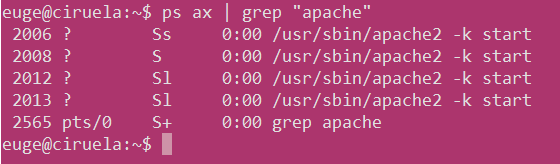
\includegraphics[scale=0.6]{Images/Apache/fig1.png}
   			\caption{\texttt{ps ax | grep ``apache''}}
    			\label{fig:1}
		\end{figure}

		Antes de proceder, debimos asegurarnos de no tener un servidor web corriendo en Windows. Si hubi'eramos tenido uno, habr'iamos tenido un problema: los protocolos HTTP usan, por defecto, el puerto TCP 80; si el puerto est'a en uso (si tuvi'eramos otro servidor web), tendr'iamos que redireccionar los puertos y llevar'ia m'as trabajo.

		Una forma de asegurarnos de que el puerto 80 est'a libre es correr en el sistema \texttt{telnet localhost 80}. Telnet, como contamos previamente, es un programa que nos permite conectarnos a una computadora remota. La sintaxis de este comando es as'i: \texttt{telnet <servidor>{} <puerto>}. Es decir, al escribir \texttt{telnet localhost 80}, le estamos pidiendo a la computadora que se conecte a su puerto 80. Este paso debe realizarse desde la consola de Windows, no en la m'aquina virtual.

		Algo a resaltar es que es probable que el servicio \texttt{telnet} est'e desactivado en Windows. Para activarlo, simplemente buscamos entre las aplicaciones ``\texttt{Activar o desactivar caracter'isticas de Windows}'' y tildamos el casillero que dice ``\texttt{Telnet Client}''. 

		\begin{figure}[H]
  			\centering \captionsetup{justification=centering}
    			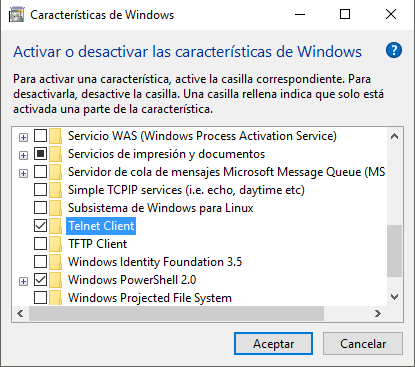
\includegraphics[scale=0.65]{Images/Apache/fig3.png}
    			\label{fig:3}
    			\caption{Activamos Telnet Client}
		\end{figure}

		Una vez activada esta función, ejecutamos el comando nombrado anteriormente y, si recibimos un error como ``No se puede abrir la conexi'on al host'', quiere decir que no tenemos un servidor web corriendo en este momento en Windows (m'as especificamente, que no estamos usando el puerto 80) y que podremos continuar sin problemas.

		\begin{figure}[H]
    			\centering \captionsetup{justification=centering}
    			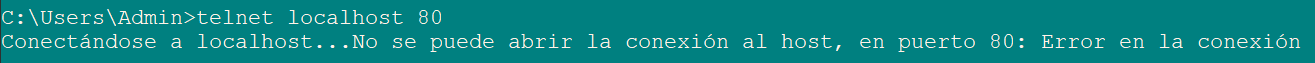
\includegraphics[scale=0.358]{Images/Apache/fig__.png}
    			\label{fig:7}
    			\caption{Mensaje en la consola al correr \texttt{telnet localhost 80}}
		\end{figure} 

		En nuestra m'aquina virtual corremos \texttt{telnet localhost 80} (ahora nos conectamos al puerto 80 de la Virtual Box) y escribimos \texttt{GET / HTTP/1.1}. Presionamos la tecla \texttt{enter} una vez y escribimos \texttt{Host: localhost}. La respuesta deber'ia ser similar a la que se muestra en la imagen \ref{fig:4}.

		\begin{table}[H]
    			\centering
    			\begin{tabular}{|l|}
        			\hline
        			\texttt{GET / HTTP/1.1} \\
        			\texttt{Host: localhost} \\\hline
    			\end{tabular}
    			\label{tab:my_label}
		\end{table}

		\begin{figure}[H]
    			\centering \captionsetup{justification=centering}
    			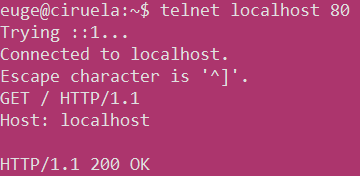
\includegraphics[scale=0.6]{Images/Apache/fig4_.png}
    			\caption{Pedimos al servidor que nos muestre la p'agina ``/'' y le indicamos que nos comunicamos en HTTP/1.1}
    			\label{fig:4}
		\end{figure}

		Pero ¿qu'e hace el comando ``\texttt{GET / HTTP/1.1}''? \texttt{GET} le pide al servidor el contenido de la p'agina \texttt{/} (una p'agina que es generada por defecto). El 'ultimo argumento que indicamos, \texttt{HTTP/1.1}, es el protocolo y la versi'on del mismo con los que nos comunicamos como cliente. 
Debemos recordar que el pedido que hace el navegador debe ser comprendido por el servidor web. Es decir, deben funcionar en el mismo protocolo: \texttt{HTTP}.
Como primera parte de la respuesta obtuvimos ``\texttt{HTTP/1.1 200 OK}'', que indica que el servidor usa, en este caso, el mismo protocolo que nosotrxs y que nos entiende. La otra parte (no visible en la figura anterior), es el c'odigo \texttt{html} de nuestra p'agina.

		Debemos recordar indicar el \texttt{Host} porque es un requisito de esta versi'on del protocolo y, de lo contrario, obtedr'iamos el error ``\texttt{Bad request}'', el servidor no nos entender'ia. Por otro lado, si escribi'eramos \texttt{GET / HTTP/1.0}, al ser una versi'on m'as vieja, no ser'ia necesario este segundo paso y se entablar'ia la comunicaci'on correctamente, como puede observarse en la figura \ref{fig:5}.

		\begin{figure}[H]
    			\centering \captionsetup{justification=centering}
    			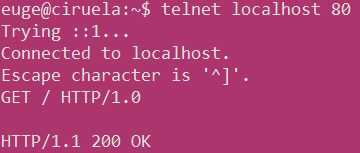
\includegraphics[scale=0.6]{Images/Apache/fig5_.png}
    			\caption{Pedimos al servidor que nos muestre la p'agina ``/'' y le indicamos que nos comunicamos en HTTP/1.0}
    			\label{fig:5}
		\end{figure}

		S'olo queda configurar los puertos de nuestra m'aquina virtual para que el servidor sea accesible desde otras m'aquinas. Para eso iremos a la aplicaci'on VirtualBox y crearemos una nueva regla de reenv'io de puertos, como hicimos al principio de este trabajo. En el nombre de la regla, indicamos ``Apache''. La configuramos para que tenga protocolo TCP y que los puertos de anfitr'on e invitado sean ambos el 80. Las IPs quedar'an vac'ios para que se acomoden autom'aticamente. De tener ocupado el puerto 80, deberemos de cambiar el puerto anfitri'on o host port en ingl'es (depende del idioma en que tenga configurado el sistema), a otro puerto ``raro'', como hicimos con SSH (pero distinto del usado all'i).

		\begin{figure}[H]
    			\centering \captionsetup{justification=centering}
    			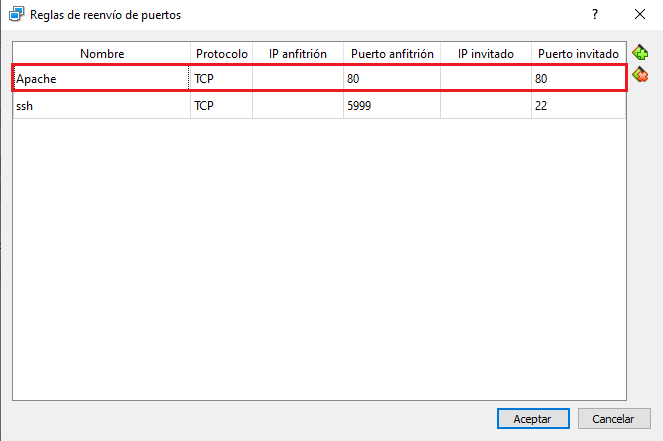
\includegraphics[scale=0.65]{Images/Apache/fig6.png}
   			\caption{Configuraci'on de reenvío de puertos para poder acceder al servidor de la VM desde el host}
    			\label{fig:6}
		\end{figure}

		Por 'ultimo, entrando a un navegador y usando la direcci'on \verb|http://localhost| o simplemente \verb|localhost| (tanto en Windows como en la m'aquina virtual), podremos verificar que todo est'e andando bien (en la pantalla dir'a inicialmente  ``It works!'', despu'es podremos editarlo). Agregar que, de haber tenido el puerto 80 ocupado y haber utilizado un puerto anfitri'on distinto, el link a ingresar en el navegador ser'ia tambi'en empezando con \verb|localhost|, pero luego seguido de dos puntos, y el puerto que hayamos asignado, como algo de la forma \texttt{http://localhost:\emph{puerto}}.
		
	\begin{figure}[H]
		\centering
		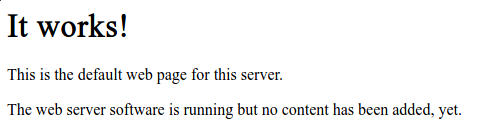
\includegraphics[width=.8\linewidth]{Images/Apache/fig7.png}
		\caption{P'agina por defecto de Apache al entrar a la direcci'on \texttt{localhost}}
		\label{fig:index_orig_code}
	\end{figure}
		
	\subsection{Transferencia de archivos y modificaci'on de la p'agina web}
	
	Ya que logramos comprobar el correcto funcionamiento de nuestra p'agina web con Apache, iremos un paso m'as all'a y modificaremos la p'agina visualizada en la direcci'on \texttt{localhost}. Para esto, y también con el fin de probar que ser'iamos capaces de almacenar archivos en nuestro servidor y modificarlos de forma remota, haremos uso de otro programa llamado WinSCP, que tambi'en hace uso del protocolo SSH.
	
	\subsubsection{Instalando y configurando WinSCP}
	
	WinSCP es un programa para Windows de c'odigo abierto que permite principalmente, la transferencia de archivos de forma remota. Soporta distintos protocolos para ello, como \texttt{FTP}, \texttt{SFTP}, \texttt{SCP}, entre otros. Este 'ultimo (de sus siglas en ingl'es, \textit{Secure Copy Protocol}), es un protocolo pr'acticamente obsoleto para la transferencia de archivos que, al igual que SFTP el cual mencionamos brevemente en la secci'on de PuTTY, est'a basado en el protocolo \texttt{SSH}. SFTP es mucho m'as completo que SCP, permitiendo comandos como renombrar archivos, eliminar, mover, entre otros, que permiten en general poder visualizar el sistema de archivos del sistema al que uno se conecte y manejarlo con mayor flexibilidad, mientras SCP simplemente es capaz de transferir archivos. Por esta raz'on, dado que ya hemos configurado una conexi'on por SSH correctamente, podremos lograr nuestro objetivo sin mayores cambios en la VM, haciendo uso por comodidad del protocolo m'as moderno, SFTP.
	%\footnote{\url{https://winscp.net/eng/download.php}} 
	% Poner el link estaría bueno, pero ponerlo genera muchos espacios por las imágenes. Si quieren veanlo cómo ponerlo
	
	Entonces, descargamos el programa desde la p'agina oficial y lo instalamos. Durante el proceso de instalaci'on probablemente surja un cuadro inform'andonos de la existencia de sesiones guardadas con PuTTY:
	
	\begin{figure}[H]
		\centering	\captionsetup{justification=centering}
		\subfloat[Sesiones guardadas detectadas]{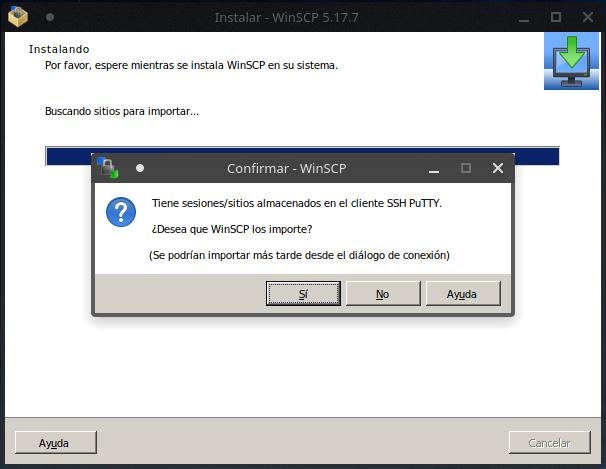
\includegraphics[width=.475\linewidth]{Images/WinSCP/fig1a}}
		\hfill
		\subfloat[Selecci'on de sesiones a importar]{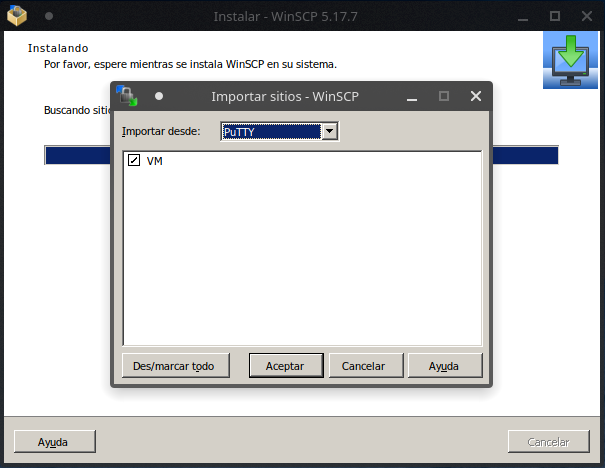
\includegraphics[width=.475\linewidth]{Images/WinSCP/fig1b}} \vspace{7pt}
		\caption{Importaci'on de sesiones guardadas desde PuTTY}
	\end{figure}

	El instalador de WinSCP detecta y permite importar sesiones guardadas previamente en PuTTY. Esto nos facilita a'un m'as el proceso de configuraci'on, ya que no es necesario indicar nuevamente el puerto, la direcci'on, o la ruta de la llave privada como tuvimos que hacerlo con PuTTY, pues justamente utilizamos las opciones previamente establecidas en dicha ocasi'on, a lo que aceptamos e importamos la sesi'on relacionada a la conexi'on con la VM.
	
	Una vez finalizada la instalaci'on, abrimos el programa en cuesti'on, y al ingresar nos pedir'a los datos de conexi'on, pero tambi'en se encuentra listada la sesi'on antes importada, que utilizamos y procedemos a conectarnos a la VM (obviamente prendida).
	
	\begin{figure}[H]
		\centering \captionsetup{justification=centering}
		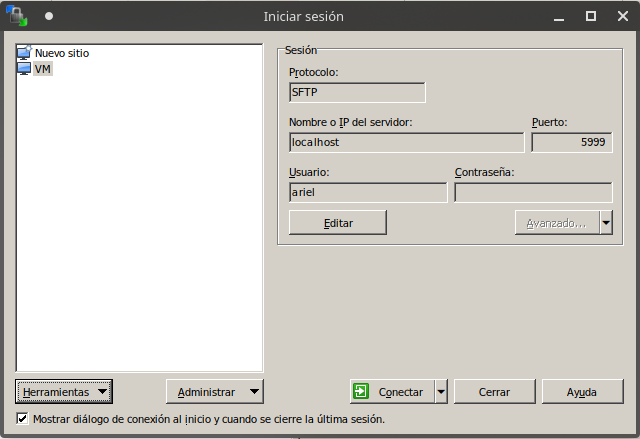
\includegraphics[width=.8\linewidth]{Images/WinSCP/fig2}
		\caption{Elegimos la sesi'on importada al abrir WinSCP}
	\end{figure}

	Una vez conectados correctamente, de haber elegido el estilo de la interfaz por defecto durante la instalaci'on, habr'an dos paneles en pantalla. En el izquierdo podremos navegar por el sistema de archivos de la computadora \emph{desde} la que nos conectamos, y en el derecho por el de la computadora \emph{a la cual} nos conectamos.
	
	\begin{figure}[H]
		\centering \captionsetup{justification=centering}
		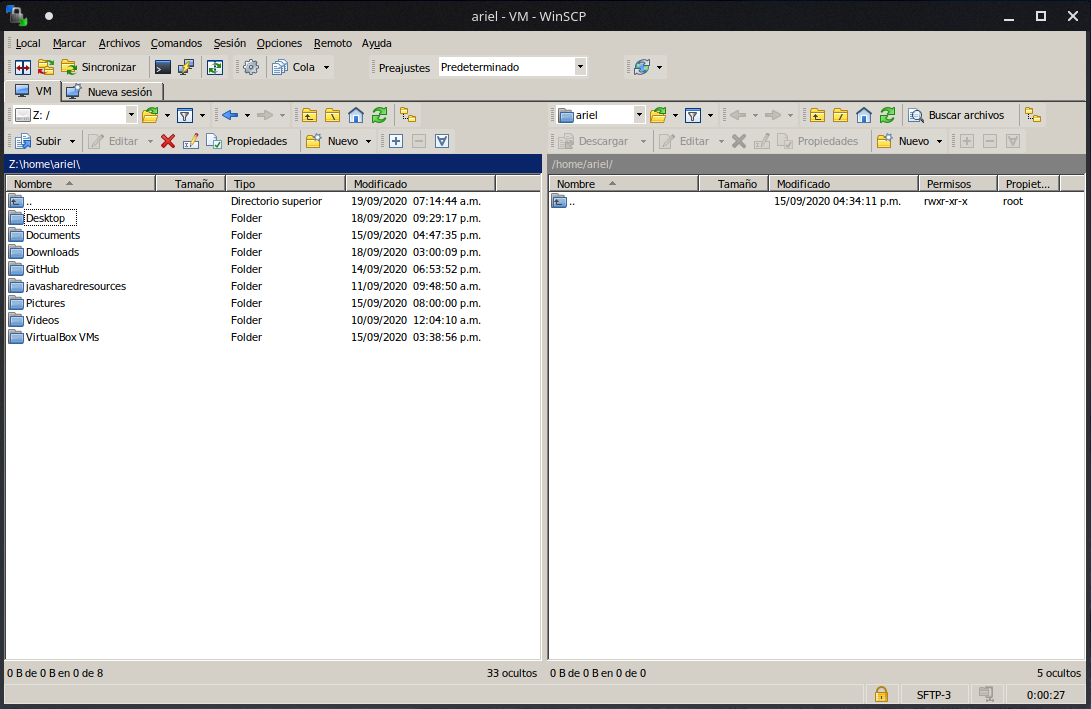
\includegraphics[width=.8\linewidth]{Images/WinSCP/fig3}
		\caption{Podemos ver los archivos de las m'aquinas a ambos extremos de la conexi'on}
	\end{figure}

	\subsubsection{Modificando la p'agina web}

	La p'agina web que muestra Apache por defecto, que vimos en una secci'on anterior, se encuentra almacenada en la ruta \verb|/var/www/index.html| (por supuesto, en este caso, dentro de la VM). Por lo tanto, si queremos modificar los contenidos de dicha p'agina, los cambios a aplicar ser'an en principio, sobre el archivo en cuesti'on. Notar la extensi'on \texttt{.html}, que por convenci'on, determinar'ia que su contenido es c'odigo en el lenguaje HTML. De sus siglas en inglés, el \textit{HyperText Markup Language} es un lenguaje est'andar para la definici'on del contenido de una p'agina web. Es decir, si queremos hacer cambios sobre el archivo \texttt{index.html}, tendremos que respetar las pautas de este lenguaje para que nuestros cambios sean correctamente comprendidos por un navegador web. 
	
	El contenido original de \texttt{index.html} se puede ver en la sección de Código utilizado. 
	
	Entonces, investigamos sobre el uso de HTML y confeccionamos un nuevo archivo \texttt{index.html} que transferimos a la máquina virtual para cambiar lo que se visualiza en la p'agina web. Para ello, en WinSCP buscamos nuestro archivo dentro de la computadora de origen en el panel izquierdo, y en el panel derecho entramos a la ruta de \texttt{index.html} antes mencionada, y arrastramos el archivo a transferir de un panel al otro. Cuando nos pregunta si queremos sobreescribir un archivo existente aceptamos (pues los nombres son iguales), pero luego nos encontramos con un inconveniente:
	
	\begin{figure}[H]
		\centering \captionsetup{justification=centering}
		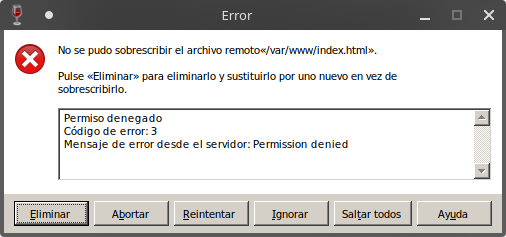
\includegraphics[width=.8\linewidth]{Images/WinSCP/fig4}
		\caption{Error al querer transferir nuestro nuevo archivo \texttt{index.html} a \texttt{/var/www} en la VM}
	\end{figure}

	Resulta que el archivo generado por Apache, al haber sido este 'ultimo instalado con permisos de superusuario (\texttt{\emph{\textbf{sudo}} apt-get install...}), el due'no de tal archivo es el usuario \texttt{\emph{root}}, por lo que al acceder con WinSCP a trav'es de nuestro usuario, no tenemos permisos suficientes para ejercer cambios sobre \texttt{index.html} en la VM.
	
	Para solucionarlo, hacemos uso del comando \texttt{chown} que, como hemos visto en trabajos pr'acticos pasados, permite cambiar el ``due'no'' de un archivo. Y por supuesto, tendremos que hacerlo en combinaci'on con \texttt{sudo}, al ser el due'no original, \texttt{\emph{root}}. El comando final ser'ia entonces (y ya que tenemos abierta la terminal con PuTTY, lo ejecutaremos a trav'es de ella)  \verb|sudo chown nuestroUsuario /var/www/index.html|. De esta forma, al volver a intentar transferir el archivo, podemos hacerlo sin problemas.
	
	\begin{figure}[H]
		\centering \captionsetup{justification=centering}
		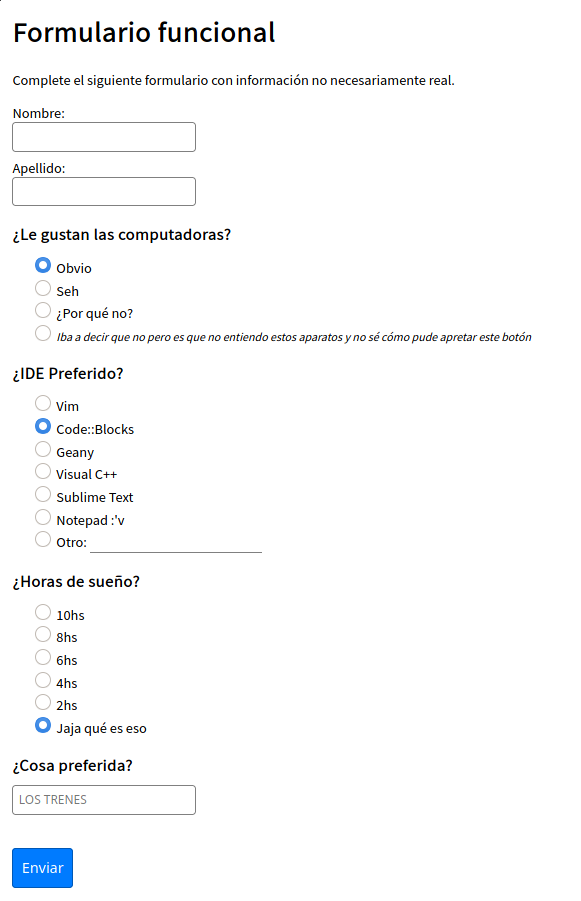
\includegraphics[width=.55\linewidth]{Images/WinSCP/fig5}
		\caption{Vista de la p'agina web despu'es de haber transferido nuestro archivo \texttt{index.html} a la VM}
		\label{fig:index_ours_code}
	\end{figure}

	Entonces, ahora al acceder de nuevo a la direcci'on \texttt{localhost} desde el host de la VM, podemos efectivamente comprobar que nos muestra el \texttt{index.html} que hicimos, y funciona sin problemas.

	Se puede encontrar el archivo  \texttt{index.html} que hicimos tambi'en en la secci'on de C'odigo utilizado.
		
	\section{Comandos usados}
		A continuaci'on se encuentran todos los comandos utilizados en este trabajo, correspondientes a las im'agenes presentadas.
		
		\begin{figure}[H]
			\centering
			\begin{code-box}
				\codetext{light-blue}{ps} \codetext{light-orange}{ax} \textbar\/ \codetext{light-blue}{grep} \codetext{light-red}{``ssh''}
				
				\codetext{light-blue}{/etc/init.d/ssh} \codetext{light-orange}{status}
			\end{code-box}
			\imagecaption{SSH_check}
		\end{figure}
		
		\begin{figure}[H]
			\centering
			\begin{code-box}
				\codetext{dark-gray}{---- BEGIN SSH2 PUBLIC KEY ----\\
				Comment: ``rsa-key-20200831''\\
				AAAAB3NzaC1yc2EAAAABJQAAAQEAhkS24rsmFKN63BDW+BpZZVkcl
				z64xRfa2dPeAdJVp6wJzo23oEizBxKs2/OIOE2/2uQ22sThb1Gi5j
				rRvZQRFwAtiRPygwlEd0pzcFortg+G9x98iZwYnA317Hh8il1JrNy
				ZamEsZNzchpAwXYlaXI92jY3ABsC5HGDGNMK3rS63hsgArgpKjCZS
				5+IftXJLAxjhgSXSS0bbf5bJ3KkBtjghRmKCibm6b/zbBrjVN1ms1
				HLBbofNbtgPmXjLlMtXB6wWfmz4epySU9lRY4Qqbr/zuW+GrbpdRo
				8T40xls8S06pqfro8om7jubGoCBO/t2rEGgniaNihUbs3VOQ74TQ==\\
				---- END SSH2 PUBLIC KEY ----}
			\end{code-box}
			\imagecaption{public_key}
		\end{figure}
		
		\begin{figure}[H]
			\centering
			\begin{code-box}
				\codetext{fuchsia}{sudo} \codetext{light-blue}{/etc/init.d/ssh} \codetext{light-orange}{restart}
			\end{code-box}
			\imagecaption{ssh_restart}
		\end{figure}
		
		\begin{figure}[H]
			\centering
			\begin{code-box}
				\codetext{dark-gray}{ssh-rsa AAAAB3NzaC1yc2EAAAABJQAAAQEAhkS24rsmFKN63BDW+
				BpZZVkclz64xRfa2dPeAdJVp6wJzo23oEizBxKs2/OIOE2/2uQ22s
				Thb1Gi5jrRvZQRFwAtiRPygwlEd0pzcFortg+G9x98iZwYnA317Hh
				8il1JrNyZamEsZNzchpAwXYlaXI92jY3ABsC5HGDGNMK3rS63hsgA
				rgpKjCZS5+IftXJLAxjhgSXSS0bbf5bJ3KkBtjghRmKCibm6b/zbB
				rjVN1ms1HLBbofNbtgPmXjLlMtXB6wWfmz4epySU9lRY4Qqbr/zuW
				+GrbpdRo8T40xls8S06pqfro8om7jubGoCBO/t2rEGgniaNihUbs3
				VOQ74TQ==}
			\end{code-box}
			\imagecaption{public_key_final}
		\end{figure}
		
		\begin{figure}[H]
			\centering
			\begin{code-box}
				\codetext{fuchsia}{sudo } \codetext{light-blue}{apt-get } \codetext{light-orange}{install } \codetext{dark-gray}{apache2}
			\end{code-box}
			\imagecaption{1}
		\end{figure}
		
		\begin{figure}[H]
			\centering
			\begin{code-box}
				\codetext{light-blue}{ps } \codetext{light-orange}{ax } \codetext{dark-gray}{| } \codetext{light-blue}{grep } \codetext{dark-gray}{``apache''}
			\end{code-box}
			\imagecaption{1}
		\end{figure}

		\begin{figure}[H]
			\centering
			\begin{code-box}
				\codetext{light-blue}{telnet } \codetext{light-orange}{localhost 80}
			\end{code-box}
			\imagecaption{7}
		\end{figure}
		
		\begin{figure}[H]
			\centering
			\begin{code-box}
				\codetext{light-blue}{telnet } \codetext{light-orange}{localhost 80}\newline
				\codetext{light-blue}{GET } \codetext{light-orange}{/ HTTP/1.1}\newline
				\codetext{light-blue}{Host: } \codetext{dark-gray}{localhost}
			\end{code-box}
			\imagecaption{4}
		\end{figure}
	
	\section{C'odigo utilizado}
	
	\lstset{style=HTML}
	\lstinputlisting[language=HTML, title=\char91\ref{fig:index_orig_code}\char93\:{}Archivo original \texttt{index.html}]{Resources/WinSCP/index.html}
	
	\lstinputlisting[language=HTML, title=\char91\ref{fig:index_ours_code}\char93\:{}Nuestro nuevo archivo \texttt{index.html}]{Resources/WinSCP/index-ours.html}
























%Remove whitspace when done, for ease of work.
\end{document}
